% Input common header
\documentclass[xcolor=dvipsnames]{beamer}

\usecolortheme[named=Blue]{structure}
\setbeamertemplate{itemize items}[circle]

\usepackage{smartdiagram}


\author{Dr. Paul Larsen}
\date{\today}


\title{Implementing Artificial Intelligence in Practice}
\begin{document}
\maketitle

\begin{frame}
\frametitle{Managing AI Model Risk: Buzzwords That Matter}
\begin{itemize}
\item Agile: \href{https://agilemanifesto.org/}{agilemanifesto.org}
\item TDD: \href{https://www.oreilly.com/library/view/test-driven-development/0321146530/}{Kent Beck, {\it Test Driven Development: By Example}}
\item DevOps: \href{https://landing.google.com/sre/books/}{Google's {\it Site Reliability Engineering}}
\end{itemize}
\begin{center}
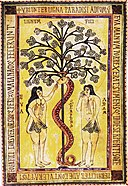
\includegraphics[height=0.35\textheight]{figures/Codex_Aemilianensis}
\end{center}
Source: \url{https://commons.wikimedia.org/wiki/File:Codex_Aemilianensis.jpg}
\end{frame}

\begin{frame}
\frametitle{Standard Model Metrics (Almost) Never Matter}
\end{frame}

\begin{frame}
\frametitle{The Biggest Danger Posed by AI is Dishonest Practitioners}
Either (likely) unknowlingly: https://peerj.com/articles/cs-93/

Or (possibly) knowingly: ???
\end{frame}

% \begin{frame}
% \frametitle{Forrest Gump was Right About AI}
% \begin{itemize}
% \item AI is as AI does
% \item AI is like a box of chocolates, you never know what you're gonna get
% \end{itemize}
% \end{frame}

\begin{frame}
\frametitle{Is deploying AI different?}

No, since it is still is software
\begin{itemize}
\item Manage dependencies (e.g. workshop material, polytope packages)
\item Library + app
\end{itemize}

Yes, since it is not standard software
\begin{itemize}
    \item Python
    \item Model maintenance
\end{itemize}
\end{frame}

\begin{frame}
\frametitle{Making AI Work for Enterprise, Another Sports Analogy}
\begin{itemize}
\item Minimize friction
\item Work smart
\end{itemize}
\end{frame}
\end{document}